\documentclass[dvipsnames,handout]{beamer} % Use handout option to remove pauses.
\usetheme{default}
\usefonttheme{structurebold}
\usefonttheme[onlymath]{serif}
\usepackage[UKenglish,cleanlook]{isodate}                                  % Set default date and date display
\usepackage[T1]{fontenc}
% Slide title background color
\definecolor{background}{HTML}{ede6d8}
% Slide title text color
\definecolor{titleText}{HTML}{B40404}
% and for structural objects
% Add slide numbers in bottom right corner
\defbeamertemplate{headline}{my header}{
    \vskip1pt
    \makebox[0pt][l]{\,\insertsection}
    \hspace*{\fill}\insertshorttitle\hspace*{\fill}
    \llap{\insertframenumber\,/\,\inserttotalframenumber\,}
}
\setbeamertemplate{headline}[my header]
% Add name at the bottom
\setbeamercolor{footlinecolor}{fg=black,bg=background}
\defbeamertemplate{footline}{my footer}{%
    \begin{beamercolorbox}[wd=\paperwidth,leftskip=0.25cm,rightskip=0.25cm]{footlinecolor}
        \insertshortauthor
        \hfill
        \insertframenumber{} / \inserttotalframenumber
    \end{beamercolorbox}
}
\setbeamertemplate{footline}[my footer]
\setbeamertemplate{navigation symbols}[default]
\usepackage{graphicx}
% Set font sizes for frame title and subtitle
\setbeamerfont{frametitle}{size=\fontsize{15}{16}}
\setbeamerfont{framesubtitle}{size=\small}
% Set left and right text margins
\setbeamersize{text margin left=5mm, text margin right=5mm}
\usepackage{booktabs,multirow}
\usepackage{subcaption}   % Sub figures.
\usepackage{tikz}
\usetikzlibrary{shapes,decorations,decorations.pathreplacing,arrows,calc,arrows.meta,fit,positioning}
\tikzset{
    auto,node distance =1 cm and 1 cm,semithick,
    state/.style ={ellipse, draw, minimum width = 0.7 cm},
    point/.style = {circle, draw, inner sep=0.04cm,fill,node contents={}},
    bidirected/.style={Latex-Latex,dashed},
    el/.style = {inner sep=2pt, align=left, sloped}
}
\usepackage{mathtools}                                                     % Various maths functions
\usepackage{amssymb}                                                       % Various maths functions
\usepackage{amsmath}                                                       % Various maths functions
\usepackage{dsfont}                                                        % Various maths functions
\usepackage{centernot}                                                     % center \not usage
\usepackage{siunitx} \sisetup{round-mode=places, round-precision=3}        % Formalise use of units and numbers among text
\usepackage[normalem]{ulem} % Strike-through package
\renewcommand{\vec}[1]{\boldsymbol{\mathit{#1}}}                           % vector notation shortcut
\newcommand{\mat}[1]{\boldsymbol{\mathit{#1}}}                             % matrix notation shortcut
\DeclarePairedDelimiter\abs{\lvert}{\rvert}                                % absolute value notation shortcut
\DeclarePairedDelimiter\norm{\lVert}{\rVert}                               % norm notation shortcut
\newcommand{\Prob}[1]{\Pr\left( #1 \right)}                         % SHortcut for probability notation
\newcommand{\Probgiven}[2]{\Pr\left( #1 \, \middle\vert \, #2 \right)} % SHortcut for probability notation, given
\newcommand{\E}[2][]{\mathbb{E}_{#1} \left[ #2 \right]}                    % Expectation (with optional subscript) shortcut
\newcommand{\Egiven}[3][]{\mathbb{E}_{#1} \left[ #2 \, \middle\vert \, #3 \right]} % Expectation given (with optional subscript) shortcut
\newcommand{\Var}[2][]{\text{Var}_{#1} \left( #2 \right)}                  % Variation (with optional subscript) shortcut
\newcommand{\Cov}[1]{\text{Cov} \left( #1 \right)}                         % Covariance (with optional subscript) shortcut
\newcommand{\indicator}[1]{\mathds{1}\left\{ #1 \right\}}                  % SHortcut for indicator function
\newcommand{\indep}{\, \raisebox{0.05em}{\rotatebox[origin=c]{90}{$\models$}} \,}% Statistical independence symbol.
\newcommand{\diff}[2][]{\frac{d#1}{d#2}}                                   % SHortcut for differential fraction as a function
\newcommand{\partialdiff}[2][]{\frac{\partial#1}{\partial#2}}              % SHortcut for partial differential fraction as a function
\renewcommand{\hat}[1]{\widehat{#1}}                                       % Default estimator notation is widehat
\renewcommand{\bar}[1]{\overline{#1}}                                      % Make over bar look nicer
\renewcommand{\tilde}[1]{\widetilde{#1}}                                   % Make over tilde look better
% Citations
\usepackage{natbib}                                        % Citation package, see https://en.wikibooks.org/wiki/LaTeX/Bibliography_Management#Natbib
\usepackage{hyperref}                                        % Allow for links across the text, with colour options
\usepackage{setspace}
\settowidth{\leftmargini}{\usebeamertemplate{itemize item}}
\addtolength{\leftmargini}{\labelsep}
\usepackage{soul,color,xcolor} % Text highlighting
\newcommand{\eqhighlight}[2]{\colorbox{#1!50}{$\displaystyle#2$}}
\makeatletter
\let\HL\hl
\renewcommand\hl{%
    \let\set@color\beamerorig@set@color
    \let\reset@color\beamerorig@reset@color
    \HL}
\makeatother
\newcommand{\mathcolorbox}[2]{\colorbox{#1}{$\displaystyle #2$}}
% Set colors
\setbeamercolor{block title}{use=structure,fg=white,bg=structure.fg!75!black}
\setbeamercolor{block body}{parent=normal text,use=block title,bg=block title.bg!10!bg}
\setbeamercovered{transparent}
\setbeamercolor{postit}{fg=black, bg=yellow}
\setbeamercolor{frametitle}{bg=background, fg=titleText}
\setbeamercolor{subtitle}{fg=titleText}
% Command to align text
\renewcommand{\raggedright}{\leftskip=0pt \rightskip=0pt plus 0cm}
% Remove the useless buttons.
\setbeamertemplate{navigation symbols}{}
\useoutertheme[footline=empty,subsection=false]{miniframes}
\useinnertheme{circles}

%-------------------------------------------------------------------------------
% Title Page
%-------------------------------------------------------------------------------
\title{\color{titleText}
    \href{https://raw.githubusercontent.com/shoganhennessy/mediation-natural-experiment/main/mediation-natural-experiment-2025.pdf}{Causal Mediation in Natural Experiments}
}
\author[Senan Hogan-Hennessy, Cornell University]{
    Senan Hogan-Hennessy \\
    Economics Department, Cornell University \\ %\vspace{0.5cm}
    \href{mailto:seh325@cornell.edu}{\textcolor{blue}{seh325@cornell.edu}}
}
\date{} % Date, can be changed to a custom date

%-------------------------------------------------------------------------------
% Opening Slides
\begin{document}
% Justify text through-out.
\raggedright
%-------------------------------------------------------------------------------
\begin{frame}
    \frametitle{Notes for long version}
    \begin{enumerate}
        \item Translate the wording for everyone (mechanism, quasi-random), and be clearer about suggestive.  Use words like necessary but not sufficient.
        \item Needs a clearer introduction, which accurately overviews and previews the approach findings
        \item Novelty needs to be loud, so put it first, Write ATE $=$ ADE $+$ AIE for Levon, and enumerates folks theorems for why CM did not take off in econ but did in medicine epi psych)
        \item Evan Riehl recommends a slide with quotes from top 5s that investigates mechanisms (note the approach is necessary but not sufficient for mechanism analysis)
        \item Mention Kwon Roth result on my data, reject null then move on....
        \item Longer presentation needs clear reasoning on the IV.
    \end{enumerate}
\end{frame}
%-------------------------------------------------------------------------------
\begin{frame}
    \frametitle{Notes for long version: empirical IV}
    \begin{enumerate}
        \item Longer explanation of the IV in Oregon for applied audience
        \item Options for the included IV, mainly to consider as illustrative (and do not want people to expect a super clean IV, but then get an illustrative one).
        \item Talk through the quasi-experimental concerns (why is $D_i$ endogenous?)
        \item Show the IV set-up (clean pre-$Z_i$ first-stage, but exclusion restriction maybe lacking).  Can it be made binary to simplify the interpretation (and linearise the estimation?).
        \item Develop at least one slide that talks through the controlling for \textit{already diagnosed} illnesses
        \item See what the CM estimates look like without controlling for them already.
    \end{enumerate}
\end{frame}
%-------------------------------------------------------------------------------
%% Title page
\begin{frame}[noframenumbering, plain]
    % Print the title page as the first slide
    \vspace{1.5cm}
    \titlepage
    \begin{center}
        \vspace{-1.5cm}
        \includegraphics[width=2cm]{presentation-files/cornell}

        %\vspace{0.5cm}
        \vskip0pt plus 1filll
        \par\noindent\rule{\textwidth}{0.4pt}
        Cornell, Labor Economics Seminar \\
        17 November 2025
    \end{center}
\end{frame}

%-------------------------------------------------------------------------------
\begin{frame}
    \frametitle{Presentation Plan}
    \textbf{Introduction} \\
    First ten minutes: introduction, road-map, and preview of findings.
    \begin{itemize}
        \item Mechanism are important (show top 5 quotes), and we do not know much about them and given (at best) suggestive evidence.
        \item CM is a framework from elsewhere which gives sufficient evidence, though has not taken off in economics
        \item I give explicit reasoning for why conventional CM methods are unlikely to work in applied econ settings, then develop a structural approach to get back to what you want.
        \item Apply these methods to Oregon, showing how these methods work in practice (suggestive, conventional CM, then my MTE approach).
    \end{itemize}
    For this part, no model and no maths notation, just vibes.
\end{frame}
\begin{frame}
\frametitle{Presentation Plan}
    \textbf{1. Oregon} \\
    Second ten-minutes, the model and suggestive evidence in the OHIE.
    \begin{itemize}
        \item Introduce the OHIE, and say why the mechanisms are important and unknown
        \item Show suggestive evidence
        \item Question whether suggestive evidence is enough, when $D_i \to Y_i$ correlation is zero. 
    \end{itemize}
\end{frame}
\begin{frame}
\frametitle{Presentation Plan}
    \textbf{2. Causal Mediation} \\
    15-minutes, the CM framework. 
    \begin{itemize}
        \item Model: Define the ADE and AIE, identifying assumption, and thus sufficient evidence on this mechanism.
        \item Explain why this does not hold (e.g., Roy model), and get selection bias (figure of simulation)
        \item Show the figure of conventional CM (i.e., assume the mechanism) estimate for OHIE.  Explain why MI would not hold for Oregon
    \end{itemize}
\end{frame}
\begin{frame}
\frametitle{Presentation Plan}
    \textbf{3. CM with Selection}
    15-minutes, My approach to CM.
    \begin{itemize}
        \item Write the two-stage equation, giving intuition on where non-identification comes from (second-stage).
        \item Use my 3 assumption approach to identify the mediator mechanism MTE, then ADE $+$ AIE (write equations, and short guide, but be careful)
        \item Explain estimation with my simulation figures.
    \end{itemize}
\end{frame}
\begin{frame}
\frametitle{Presentation Plan}
    \textbf{4. Return to Oregon}
    10-minutes, my application of CM.
    \begin{itemize}
        \item Re-introduce the setting (good lottery first-stage, but hospital visits are free choice).
        \item Walk through my MTE model, with monotonicity $+$ relevance, then walk through the IV (if illustrative)
        \item Show my estimates of CM effects, then give discussion of findings.  Include an adjusted slide of not controlling for pre-diagnosed illnesses, alluding to Oster (2019) reasoning on controlling for more ailments to get a sharper answer.
    \end{itemize}
    Finding notes: very different CM effects from conventional, noting direct (psychological) effects of socialised healthcare access.
    Agreed with suggestive evidence, giving clear uncertainty on the proportion of the mechanism.
    Note $\to$ apply the Kitagawa (2015) Kwon Roth (2024) test to these data rejects null (there are direct effects). 
\end{frame}
\begin{frame}
\frametitle{Presentation Plan}
    \textbf{Conclusion}
    Bullet-point overview of everything that has happened..
\end{frame}
%-------------------------------------------------------------------------------
\section{Introduction}
\begin{frame}
    \frametitle{Causal Mediation in Natural Experiments}
    Natural experiments gives credible estimates of causal effects
    \begin{itemize}
        \item Little information on the \textcolor{ForestGreen}{mechanisms} through which they operate
        \item Limits understanding of the decisions and underlying economic system
        \item  
    \end{itemize}

    School meals $\to$ adult income, because increased education 
    (Lundborg Rooth Alex-Petersen 2022).

    \textbf{Senan note:} unsure how to start the presentation with 5 minutes that grab attention.
    Just start section 1, introducing the data succinctly.
\end{frame}
%-------------------------------------------------------------------------------
\section{1. Oregon}
\begin{frame}
    \frametitle{Oregon Health Insurance Experiment}
    In the USA, healthcare is only provided by the government in special cases

    $\to$ Medicaid is the government programme which provides health insurance for those close to the poverty line ($>70$ million people in 2025).
    \vskip-0.5cm
    \begin{figure}
        \centering
        \singlespacing
        \includegraphics[width=0.75\textwidth]{figures/medicaid-nyt.png}
    \end{figure}
\end{frame}
%-------------------------------------------------------------------------------
\begin{frame}
    \frametitle{Oregon Health Insurance Experiment}
    In the USA, healthcare is only provided by the government in special cases

    $\to$ Medicaid is the government programme which provides health insurance for those close to the poverty line ($>70$ million people in 2025).
    \begin{figure}
        \centering
        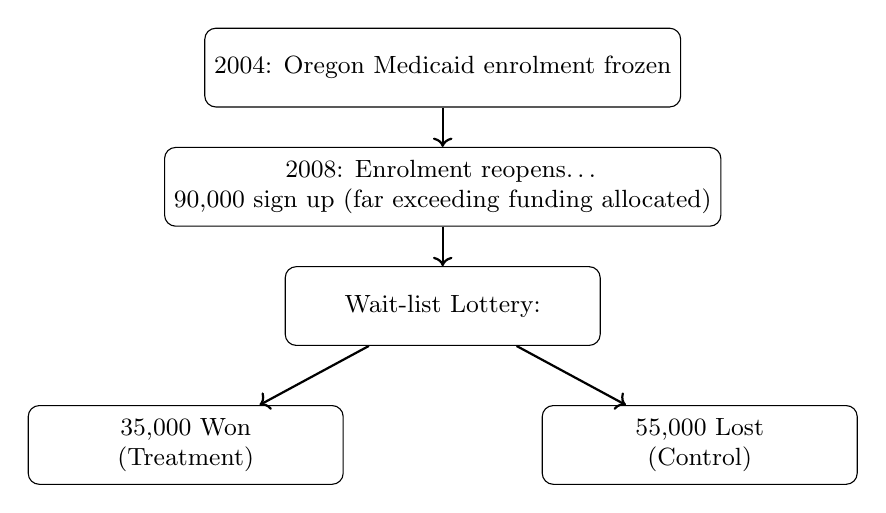
\begin{tikzpicture}[
            node distance=5mm,
            every node/.style={rectangle, draw, rounded corners, align=center, font=\small, minimum width=4cm, minimum height=1cm},
            arrow/.style={->, thick}]
            % Nodes
            \node (freeze) {2004: Oregon Medicaid enrolment frozen};
            \node (reopen) [below=of freeze] {2008: Enrolment reopens\dots \\ 90,000 sign up (far exceeding funding allocated)};
            \pause
            \node (lottery) [below=of reopen] {Wait-list Lottery:};
            \node (treat) [below left=7.5mm and -7.5mm of lottery] {35,000 Won \\ (Treatment)};
            \node (control) [below right=7.5mm and -7.5mm of lottery] {55,000 Lost \\(Control)};
            % Arrows
            \draw[arrow] (freeze) -- (reopen);
            \draw[arrow] (reopen) -- (lottery);
            \draw[arrow] (lottery) -- (treat);
            \draw[arrow] (lottery) -- (control);
        \end{tikzpicture}
    \end{figure}
\end{frame}
%-------------------------------------------------------------------------------
\begin{frame}
    \frametitle{Oregon Health Insurance Experiment}
    Winning this wait-list lottery significantly increased healthcare usage, plus subjective health and well-being (Finkelstein et al, 2012).
    \vskip-0.25cm
    \begin{figure}
        \centering
        \singlespacing
        \includegraphics[width=0.8\textwidth]{
            ../text/sections/figures/insurance-effects.png}
    \end{figure}
\end{frame}
%-------------------------------------------------------------------------------
\begin{frame}
    \frametitle{Oregon --- Suggestive Evidence}
    Winning this wait-list lottery significantly increased healthcare usage, plus subjective health and well-being (Finkelstein et al, 2012).
    \begin{figure}
        %\caption{Model for Suggestive Evidence of a Mechanism.}
        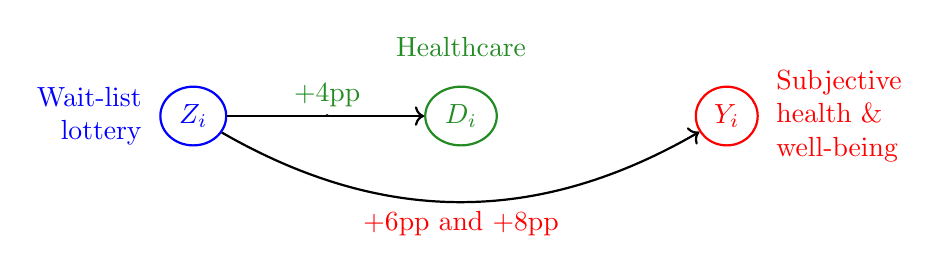
\begin{tikzpicture}
            \node[state,thick,ForestGreen] (mediator) at (0,0) {$D_i$};
            \node[state,thick,blue] (treatment) [left=2.5cm of mediator] {$Z_i$};
            \node[state,thick,red] (outcome)   [right=2.5cm of mediator] {$Y_i$};
            % Label Z_i, D, Y_i
            \node[color=ForestGreen] [above=0.25cm of mediator] {Healthcare};
            \node[color=blue,align=right] [left=0.1cm of treatment] {Wait-list \\ lottery};
            \node[color=red,align=left] [right=0.1cm of outcome] {Subjective \\ health \& \\ well-being};
            % Label the effect sizes.
            \pause
            \path[->, thick] (treatment) edge (mediator);
            \node[color=black] (firststage) at ($(mediator)!0.5!(treatment)$) {.};
            \node[color=ForestGreen] [above=-0.15cm of firststage] {+4pp};
            \pause
            \node[color=red] [below=0.7cm of mediator] {+6pp and +8pp};
            \path[->, thick] (treatment) edge[bend right=30] (outcome);
        \end{tikzpicture}
    \end{figure}
    \par\noindent\rule{\textwidth}{0.4pt}
    \vskip-0.125cm
    \pause
    \textbf{Suggestive evidence:}
    \begin{itemize}
        \item If first-stage $\neq 0$, then \textcolor{ForestGreen}{healthcare} may be a mediating mechanism
        \item This gives \textbf{suggestive evidence for \textcolor{ForestGreen}{healthcare} as mechanism}.
    \end{itemize}
\end{frame}
%-------------------------------------------------------------------------------
\begin{frame}
    \frametitle{Oregon --- Suggestive Evidence}
    \textbf{Suggestive evidence} is primarily how economics investigates mechanisms.

    \pause
    \begin{block}{Abstract --- Lundborg Rooth Alex-Petersen (2022, ReStud).} 
        ``\textellipsis Exposure to the [free school meals] programme also had substantial effects on \colorbox{yellow}{educational attainment and health}, which can \colorbox{yellow}{explain a large part of the effect} of the programme on lifetime income.''
    \end{block}

    \pause
    \begin{block}{Abstract --- Bloom Mahajan McKenzie Roberts (2013, QJE).} 
        ``\textellipsis We find that adopting these
        management practices had three main effects. First, it raised average productivity by 11\% 
        \colorbox{yellow}{through improved  quality and efficiency and reduced inventory}[\textellipsis].''
    \end{block}

    \pause
    \begin{block}{Abstract --- Carvhalo (2025, JPE Micro).} 
        ``\textellipsis \colorbox{yellow}{Evidence suggests fluid intelligence and self-control partly mediate} the relationship between the [education polygenic index] and education.''
    \end{block}
\end{frame}
%-------------------------------------------------------------------------------
\begin{frame}
    \frametitle{Oregon --- Suggestive Evidence}
    Winning this wait-list lottery significantly increased healthcare usage, plus subjective health and well-being (Finkelstein et al, 2012).
    \begin{figure}
        %\caption{Model for Suggestive Evidence of a Mechanism.}
        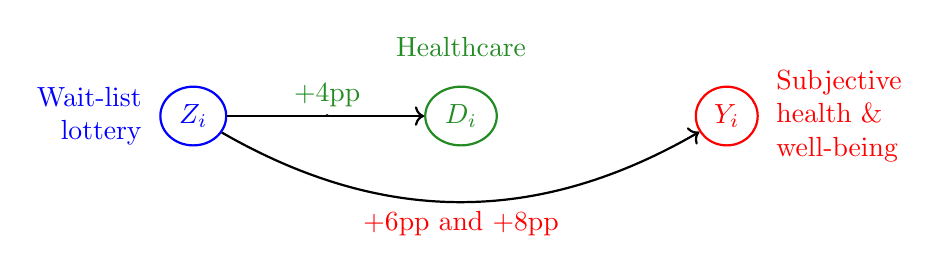
\begin{tikzpicture}
            \node[state,thick,ForestGreen] (mediator) at (0,0) {$D_i$};
            \node[state,thick,blue] (treatment) [left=2.5cm of mediator] {$Z_i$};
            \node[state,thick,red] (outcome)   [right=2.5cm of mediator] {$Y_i$};
            % Label Z_i, D, Y_i
            \node[color=ForestGreen] [above=0.25cm of mediator] {Healthcare};
            \node[color=blue,align=right] [left=0.1cm of treatment] {Wait-list \\ lottery};
            \node[color=red,align=left] [right=0.1cm of outcome] {Subjective \\ health \& \\ well-being};
            % Label the effect sizes.
            \path[->, thick] (treatment) edge (mediator);
            \node[color=black] (firststage) at ($(mediator)!0.5!(treatment)$) {.};
            \node[color=ForestGreen] [above=-0.15cm of firststage] {+4pp};
            \node[color=red] [below=0.7cm of mediator] {+6pp and +8pp};
            \path[->, thick] (treatment) edge[bend right=30] (outcome);
        \end{tikzpicture}
    \end{figure}
    \par\noindent\rule{\textwidth}{0.4pt}
    \vskip-0.125cm
    \pause
    \textbf{What about direct effects?}
    \begin{itemize}
        \item Winning access to Medicaid means you can file for free health insurance (income effect)
        \item Less stress from no longer having to be uninsured (psychological gains).
    \end{itemize}
\end{frame}
%-------------------------------------------------------------------------------
\begin{frame}
    \frametitle{Oregon --- Suggestive Evidence}
    Winning this wait-list lottery significantly increased healthcare usage, plus subjective health and well-being (Finkelstein et al, 2012).
    \begin{figure}
        %\caption{Model for Suggestive Evidence of a Mechanism.}
        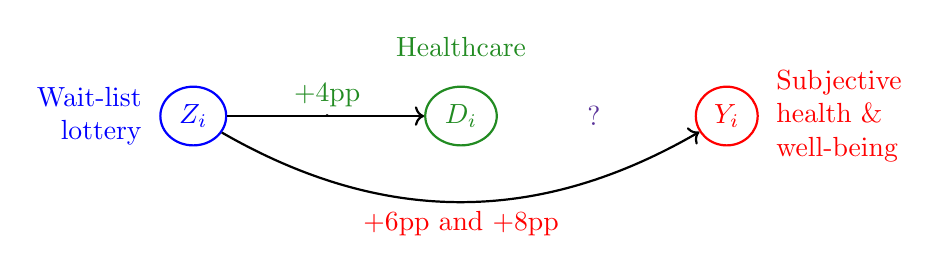
\begin{tikzpicture}
            \node[state,thick,ForestGreen] (mediator) at (0,0) {$D_i$};
            \node[state,thick,blue] (treatment) [left=2.5cm of mediator] {$Z_i$};
            \node[state,thick,red] (outcome)   [right=2.5cm of mediator] {$Y_i$};
            % Label Z_i, D, Y_i
            \node[color=ForestGreen] [above=0.25cm of mediator] {Healthcare};
            \node[color=blue,align=right] [left=0.1cm of treatment] {Wait-list \\ lottery};
            \node[color=red,align=left] [right=0.1cm of outcome] {Subjective \\ health \& \\ well-being};
            % Label the effect sizes.
            \path[->, thick] (treatment) edge (mediator);
            \node[color=black] (firststage) at ($(mediator)!0.5!(treatment)$) {.};
            \node[color=ForestGreen] [above=-0.15cm of firststage] {+4pp};
            \node[color=red] [below=0.7cm of mediator] {+6pp and +8pp};
            \path[->, thick] (treatment) edge[bend right=30] (outcome);
            \pause
            \node[color=RoyalPurple] (indirect) at ($(mediator)!0.5!(outcome)$) {?};
        \end{tikzpicture}
    \end{figure}
    \par\noindent\rule{\textwidth}{0.4pt}
    \vskip-0.125cm
    There is one missing piece to make a \textbf{definitive conclusion}:
    \[ \text{Size of causal effect }
    \textcolor{ForestGreen}{D_i} \to \textcolor{red}{Y_i} \hdots \]
    \vskip-0.125cm
    \begin{itemize}
        \item If large, then \textcolor{ForestGreen}{healthcare} explains all the lottery effect
        \item If small/zero then, then all \textcolor{blue}{direct} (e.g., psychological) gains.
    \end{itemize}
\end{frame}
%-------------------------------------------------------------------------------
\section{2. Causal Mediation (CM)}
\begin{frame}
    \frametitle{Causal Mediation (CM)}
    CM is an alternative framework to studying mechanisms, giving sufficient evidence on the mediating mechanism.
    \vskip-0.5cm
    \begin{figure}
        \centering
        \singlespacing
        
\begin{tikzpicture}
            \node (mediator) at (0,0) {};
            \node[state, thick,blue] (treatment) [left=2cm of mediator] {$Z_i$};
            \node[state, thick,red] (outcome) [right=2cm of mediator] {$Y_i$};
            % Label Z, D, Y
            \node[color=blue,align=right] [left=0.1cm of treatment] {Wait-list \\ lottery};
            \node[color=white] [above=0.25cm of mediator] {Healthcare};
            \node[color=red,align=left] [right=0.1cm of outcome] {Subjective \\ health \& \\ well-being};
            % Label the effect sizes.
            %\path[->, thick] (treatment) edge (mediator);
            \node[color=black] (firststage) at ($(mediator)!0.5!(treatment)$) {.};
            % Draw the causal arrows
            \path[->, thick] (treatment) edge (outcome);
            % Label direct and indirect effect
            \node[color=orange] [above=-0.125cm of mediator] {Treatment Effect (ATE)};
        \end{tikzpicture}
    \end{figure}
    Define
    \begin{itemize}
        \item \textcolor{blue}{Treatment $Z_i = 0, 1$}, wait-list lottery
        \item \textcolor{ForestGreen}{Mediator mechanism $D_i = 0, 1$}, healthcare usage
        \item \textcolor{red}{Outcome $Y_i$}, subjective health and well-being.
    \end{itemize}
    \par\noindent\rule{\textwidth}{0.4pt}
    CM aims to decompose the ATE in two channels, direct and indirect effects
    \[ \textcolor{orange}{\text{ATE}}
    = \textcolor{blue}{\text{ADE}} + \textcolor{ForestGreen}{\text{AIE}}. \]
\end{frame}
%-------------------------------------------------------------------------------
\begin{frame}
    \frametitle{Causal Mediation (CM)}
    CM is an alternative framework to studying mechanisms, giving sufficient evidence on the mediating mechanism.
    \vskip-0.5cm
    \begin{figure}
        \centering
        \singlespacing
        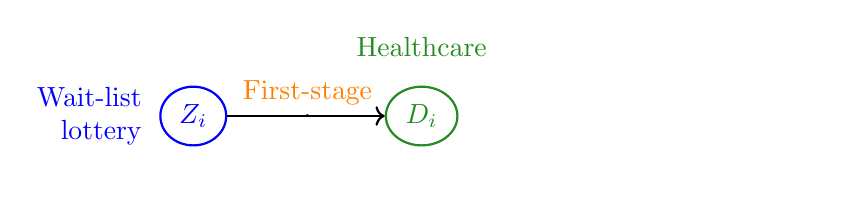
\begin{tikzpicture}
            \node[state,thick,ForestGreen] (mediator) at (0,0) {$D_i$};
            \node[state,thick,blue] (treatment) [left=2cm of mediator] {$Z_i$};
            \node[state,thick,white] (outcome) [right=2cm of mediator] {$Y_i$};
            % Label Z, D, Y
            \node[color=blue,align=right] [left=0.1cm of treatment] {Wait-list \\ lottery};
            \node[color=ForestGreen] [above=0.25cm of mediator] {Healthcare};
            \node[color=white,align=left] [right=0.1cm of outcome] {Subjective \\ health \& \\ well-being};
            % Draw the causal arrows
            \node (firststage) at ($(mediator)!0.5!(treatment)$) {.};
            \node[color=orange] [above=-0.125cm of firststage] {First-stage};
            \path[->, thick] (treatment) edge (mediator);
            % Label direct and indirect effect
            %\node[color=orange] [above=-0.125cm of mediator] {Treatment Effect (ATE)};
        \end{tikzpicture}
    \end{figure}
    Write $\textcolor{ForestGreen}{D_i}(z')$ and $\textcolor{red}{Y_i}(z', d')$ for the potential outcomes.

    \par\noindent\rule{\textwidth}{0.4pt}
    Two average causal effects are identified, with $\textcolor{blue}{Z_i}$ randomly assigned:
    \begin{enumerate}
        \item Average first-stage
        \vskip-0.125cm
        \[ \E{ \textcolor{ForestGreen}{D_i}(1) - \textcolor{ForestGreen}{D_i}(0) }
        = \Egiven{\textcolor{ForestGreen}{D_i}}{\textcolor{blue}{Z_i} = 1}
        - \Egiven{\textcolor{ForestGreen}{D_i}}{\textcolor{blue}{Z_i} = 0} \]
        \item Average Treatment Effect (ATE)
        \[ \E{ \textcolor{red}{Y_i}(1, D_i(1)) -
            \textcolor{red}{Y_i}(0, D_i(0)) }
        = \Egiven{\textcolor{red}{Y_i}}{\textcolor{blue}{Z_i} = 1}
        - \Egiven{\textcolor{red}{Y_i}}{\textcolor{blue}{Z_i} = 0}. \]
    \end{enumerate}
\end{frame}
%-------------------------------------------------------------------------------
\begin{frame}
    \frametitle{Causal Mediation (CM)}
    CM is an alternative framework to studying mechanisms, giving sufficient evidence on the mediating mechanism.
    \vskip-0.5cm
    \begin{figure}
        \centering
        \singlespacing
        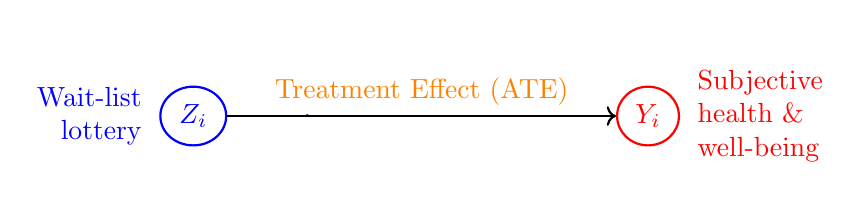
\begin{tikzpicture}
            \node[state,thick,white ] (mediator) at (0,0) {$D_i$};
            \node[state,thick,blue] (treatment) [left=2cm of mediator] {$Z_i$};
            \node[state,thick,red] (outcome) [right=2cm of mediator] {$Y_i$};
            % Label Z, D, Y
            \node[color=blue,align=right] [left=0.1cm of treatment] {Wait-list \\ lottery};
            \node[color=white] [above=0.25cm of mediator] {Healthcare};
            \node[color=red,align=left] [right=0.1cm of outcome] {Subjective \\ health \& \\ well-being};
            % Draw the causal arrows
            \node (firststage) at ($(mediator)!0.5!(treatment)$) {.};
            %\node[color=orange] [above=-0.125cm of firststage] {First-stage};
            \path[->, thick] (treatment) edge (outcome);
            % Label direct and indirect effect
            \node[color=orange] [above=-0.375cm of mediator] {Treatment Effect (ATE)};
        \end{tikzpicture}
    \end{figure}
    Write $\textcolor{ForestGreen}{D_i}(z')$ and $\textcolor{red}{Y_i}(z', d')$ for the potential outcomes.

    \par\noindent\rule{\textwidth}{0.4pt}
    Two average causal effects are identified, with $\textcolor{blue}{Z_i}$ randomly assigned:
    \begin{enumerate}
        \item Average first-stage
        \vskip-0.125cm
        \[ \E{ \textcolor{ForestGreen}{D_i}(1) - \textcolor{ForestGreen}{D_i}(0) }
        = \Egiven{\textcolor{ForestGreen}{D_i}}{\textcolor{blue}{Z_i} = 1}
        - \Egiven{\textcolor{ForestGreen}{D_i}}{\textcolor{blue}{Z_i} = 0} \]
        \item Average Treatment Effect (ATE)
        \[ \E{ \textcolor{red}{Y_i}(1, D_i(1)) -
            \textcolor{red}{Y_i}(0, D_i(0)) }
        = \Egiven{\textcolor{red}{Y_i}}{\textcolor{blue}{Z_i} = 1}
        - \Egiven{\textcolor{red}{Y_i}}{\textcolor{blue}{Z_i} = 0}. \]
    \end{enumerate}
\end{frame}
%-------------------------------------------------------------------------------
\begin{frame}
    \frametitle{Causal Mediation (CM)}
    CM is an alternative framework to studying mechanisms, giving sufficient evidence on the mediating mechanism.
    \vskip-0.5cm
    \begin{figure}
        \centering
        \singlespacing
        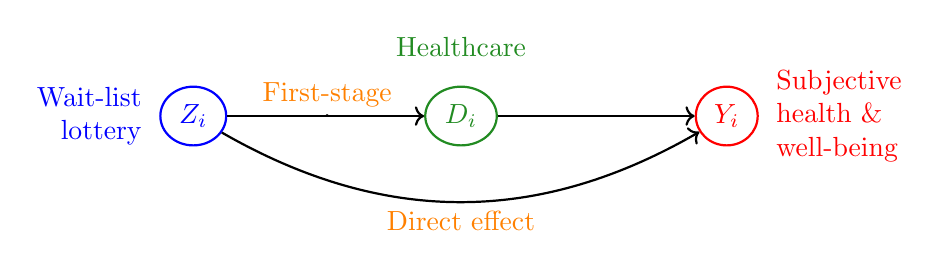
\begin{tikzpicture}
            \node[state,thick,ForestGreen] (mediator) at (0,0) {$D_i$};
            \node[state,thick,blue] (treatment) [left=2.5cm of mediator] {$Z_i$};
            \node[state,thick,red] (outcome)   [right=2.5cm of mediator] {$Y_i$};
            % Causal effects
            \path[->, thick] (treatment) edge (mediator);
            \path[->, thick] (mediator)  edge (outcome);
            \path[->, thick] (treatment) edge[bend right=30] (outcome);
            % Label Z_i, D, Y_i
            \node[color=ForestGreen] [above=0.25cm of mediator] {Healthcare};
            \node[color=blue,align=right] [left=0.1cm of treatment] {Wait-list \\ lottery};
            \node[color=red,align=left] [right=0.1cm of outcome] {Subjective \\ health \& \\ well-being};
            % Label the effect sizes.
            \node[color=black] (firststage) at ($(mediator)!0.5!(treatment)$) {.};
            \node[color=orange] [above=-0.15cm of firststage] {First-stage};
            \node[color=orange] [below=0.7cm of mediator] {Direct effect};
        \end{tikzpicture}
    \end{figure}

    \par\noindent\rule{\textwidth}{0.4pt}
    CM decomposes the ATE into components
    \[ \text{Average Indirect Effect (\textcolor{ForestGreen}{AIE})}: \;\;\;
        \E{\textcolor{red}{Y_i}\left(Z_i, \eqhighlight{ForestGreen}{D_i(1)} \right)
        -  \textcolor{red}{Y_i}\left(Z_i, \eqhighlight{ForestGreen}{D_i(0)} \right) } \]
    \textcolor{ForestGreen}{AIE} represents the average effect going \textcolor{ForestGreen}{through healthcare}.
\end{frame}%-------------------------------------------------------------------------------
\begin{frame}
    \frametitle{Causal Mediation (CM)}
    CM is an alternative framework to studying mechanisms, giving sufficient evidence on the mediating mechanism.
    \vskip-0.5cm
    \begin{figure}
        \centering
        \singlespacing
        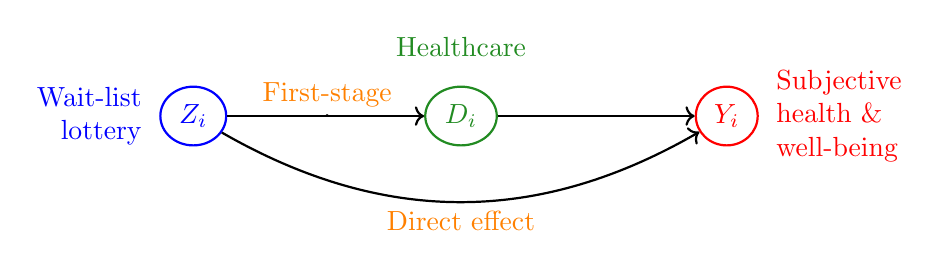
\begin{tikzpicture}
            \node[state,thick,ForestGreen] (mediator) at (0,0) {$D_i$};
            \node[state,thick,blue] (treatment) [left=2.5cm of mediator] {$Z_i$};
            \node[state,thick,red] (outcome)   [right=2.5cm of mediator] {$Y_i$};
            % Causal effects
            \path[->, thick] (treatment) edge (mediator);
            \path[->, thick] (mediator)  edge (outcome);
            \path[->, thick] (treatment) edge[bend right=30] (outcome);
            % Label Z_i, D, Y_i
            \node[color=ForestGreen] [above=0.25cm of mediator] {Healthcare};
            \node[color=blue,align=right] [left=0.1cm of treatment] {Wait-list \\ lottery};
            \node[color=red,align=left] [right=0.1cm of outcome] {Subjective \\ health \& \\ well-being};
            % Label the effect sizes.
            \node[color=black] (firststage) at ($(mediator)!0.5!(treatment)$) {.};
            \node[color=orange] [above=-0.15cm of firststage] {First-stage};
            \node[color=orange] [below=0.7cm of mediator] {Direct effect};
        \end{tikzpicture}
    \end{figure}

    \par\noindent\rule{\textwidth}{0.4pt}
    CM decomposes the ATE into components
    \[ \text{Average Direct Effect (\textcolor{blue}{ADE})}: \;\;\;
        \E{\textcolor{red}{Y_i}\left(\eqhighlight{blue}{1}, D_i(Z_i) \right)
        -  \textcolor{red}{Y_i}\left(\eqhighlight{blue}{0}, D_i(Z_i) \right)} \]
    \textcolor{blue}{ADE} represents the average effect going \textcolor{blue}{absent healthcare}.
\end{frame}%-------------------------------------------------------------------------------
\begin{frame}
    \frametitle{Causal Mediation (CM)}
    CM effects (ADE $+$ AIE) are not identified without further assumptions.
    \vskip-0.5cm
    \begin{figure}
        \centering
        \singlespacing
        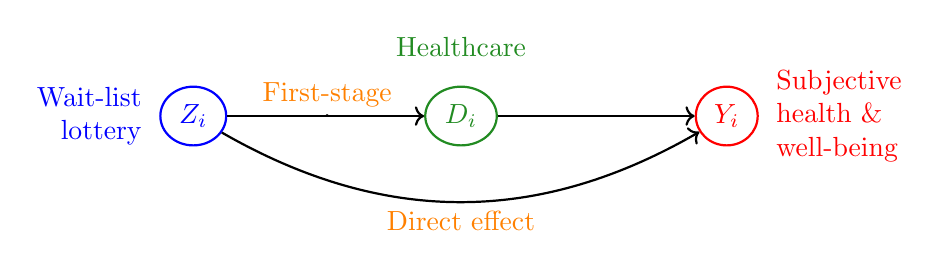
\begin{tikzpicture}
            \node[state,thick,ForestGreen] (mediator) at (0,0) {$D_i$};
            \node[state,thick,blue] (treatment) [left=2.5cm of mediator] {$Z_i$};
            \node[state,thick,red] (outcome)   [right=2.5cm of mediator] {$Y_i$};
            % Causal effects
            \path[->, thick] (treatment) edge (mediator);
            \path[->, thick] (mediator)  edge (outcome);
            \path[->, thick] (treatment) edge[bend right=30] (outcome);
            % Label Z_i, D, Y_i
            \node[color=ForestGreen] [above=0.25cm of mediator] {Healthcare};
            \node[color=blue,align=right] [left=0.1cm of treatment] {Wait-list \\ lottery};
            \node[color=red,align=left] [right=0.1cm of outcome] {Subjective \\ health \& \\ well-being};
            % Label the effect sizes.
            \node[color=black] (firststage) at ($(mediator)!0.5!(treatment)$) {.};
            \node[color=orange] [above=-0.15cm of firststage] {First-stage};
            \node[color=orange] [below=0.7cm of mediator] {Direct effect};
        \end{tikzpicture}
    \end{figure}

    \par\noindent\rule{\textwidth}{0.4pt}
    Conventional CM relies on two identifying assumptions for ADE $+$ AIE,
    \begin{enumerate}
        \item \textcolor{blue}{Treatment $Z_i$} is (quasi-)randomly assigned
        \item \textcolor{ForestGreen}{Mediator $D_i$} is (quasi-)randomly assigned, conditional on $Z_i$ realisation (and covariates $\vec X_i$).
    \end{enumerate}
\end{frame}%%-------------------------------------------------------------------------------
\begin{frame}
    \frametitle{Causal Mediation (CM)}
    Under assumptions (1) + (2), the ADE $+$ AIE are separately identified by two-stage regression (Imai Keele Yamamoto 2010).
    \begin{figure}
        \centering
        \singlespacing
        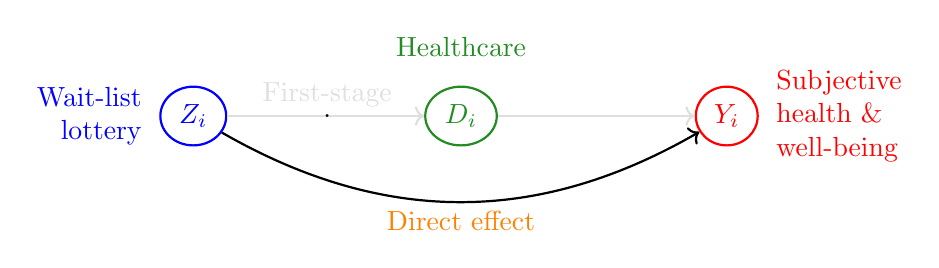
\begin{tikzpicture}
            \node[state,thick,ForestGreen] (mediator) at (0,0) {$D_i$};
            \node[state,thick,blue] (treatment) [left=2.5cm of mediator] {$Z_i$};
            \node[state,thick,red] (outcome)   [right=2.5cm of mediator] {$Y_i$};
            % Causal effects
            \path[->, thick,color=gray!25] (treatment) edge (mediator);
            \path[->, thick,color=gray!25] (mediator)  edge (outcome);
            \path[->, thick] (treatment) edge[bend right=30] (outcome);
            % Label Z_i, D, Y_i
            \node[color=ForestGreen] [above=0.25cm of mediator] {Healthcare};
            \node[color=blue,align=right] [left=0.1cm of treatment] {Wait-list \\ lottery};
            \node[color=red,align=left] [right=0.1cm of outcome] {Subjective \\ health \& \\ well-being};
            % Label the effect sizes.
            \node[color=black] (firststage) at ($(mediator)!0.5!(treatment)$) {.};
            \node[color=gray!25] [above=-0.15cm of firststage] {First-stage};
            \node[color=orange] [below=0.7cm of mediator] {Direct effect};
        \end{tikzpicture}
    \end{figure}
    \par\noindent\rule{\textwidth}{0.4pt}
    ADE is the effect of $\textcolor{blue}{Z_i}$ after controlling for $\textcolor{ForestGreen}{D_i}$
    \begin{align*}
        \textcolor{blue}{\text{ADE}}
        &= \E{\textcolor{red}{Y_i}\left(\eqhighlight{blue}{1}, D_i(Z_i) \right)
            -  \textcolor{red}{Y_i}\left(\eqhighlight{blue}{0}, D_i(Z_i) \right)} \\
        &= \Egiven{\textcolor{red}{Y_i}}{\eqhighlight{blue}{Z_i = 1}, \textcolor{ForestGreen}{D_i}}
        - \Egiven{\textcolor{red}{Y_i}}{\eqhighlight{blue}{Z_i = 0}, \textcolor{ForestGreen}{D_i}}.
    \end{align*}
\end{frame}%-------------------------------------------------------------------------------
\begin{frame}
    \frametitle{Causal Mediation (CM)}
    Under assumptions (1) + (2), the ADE $+$ AIE are separately identified by two-stage regression (Imai Keele Yamamoto 2010).
    \begin{figure}
        \centering
        \singlespacing
        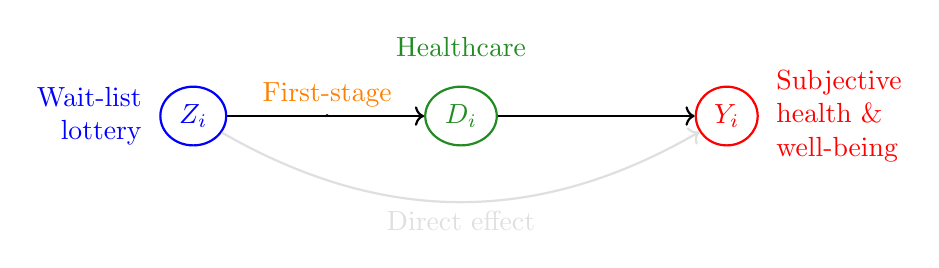
\begin{tikzpicture}
            \node[state,thick,ForestGreen] (mediator) at (0,0) {$D_i$};
            \node[state,thick,blue] (treatment) [left=2.5cm of mediator] {$Z_i$};
            \node[state,thick,red] (outcome)   [right=2.5cm of mediator] {$Y_i$};
            % Causal effects
            \path[->, thick] (treatment) edge (mediator);
            \path[->, thick] (mediator)  edge (outcome);
            \path[->, thick, color=gray!25] (treatment) edge[bend right=30] (outcome);
            % Label Z_i, D, Y_i
            \node[color=ForestGreen] [above=0.25cm of mediator] {Healthcare};
            \node[color=blue,align=right] [left=0.1cm of treatment] {Wait-list \\ lottery};
            \node[color=red,align=left] [right=0.1cm of outcome] {Subjective \\ health \& \\ well-being};
            % Label the effect sizes.
            \node[color=black] (firststage) at ($(mediator)!0.5!(treatment)$) {.};
            \node[color=orange] [above=-0.15cm of firststage] {First-stage};
            \node[color=gray!25] [below=0.7cm of mediator] {Direct effect};
        \end{tikzpicture}
    \end{figure}
    \vskip-0.5cm
    \par\noindent\rule{\textwidth}{0.4pt}
    AIE is the effect of $\textcolor{ForestGreen}{D_i}$ after controlling for
    $\textcolor{blue}{Z_i}$, times average first-stage.
    \begin{align*}
        \textcolor{ForestGreen}{\text{AIE}}
        &= \E{\textcolor{red}{Y_i}\left(Z_i, \eqhighlight{ForestGreen}{D_i(1)} \right)
        -  \textcolor{red}{Y_i}\left(Z_i, \eqhighlight{ForestGreen}{D_i(0)} \right) } \\
        &= \big(
            \Egiven{\textcolor{ForestGreen}{D_i}}{\textcolor{blue}{Z_i} = 1}
        - \Egiven{\textcolor{ForestGreen}{D_i}}{\textcolor{blue}{Z_i} = 0}\big) \\
        & \;\;\;\; \times
        \left(\Egiven{\textcolor{red}{Y_i}}{\eqhighlight{ForestGreen}{D_i = 1}, \textcolor{blue}{Z_i}}
        - \Egiven{\textcolor{red}{Y_i}}{\eqhighlight{ForestGreen}{D_i = 0}, \textcolor{blue}{Z_i}} \right).
    \end{align*}
\end{frame}%-------------------------------------------------------------------------------
\begin{frame}
    \frametitle{Causal Mediation (CM)}
    This approach (conventional CM) is used heavily in epidemiology and medicine to give evidence for the channels of a treatment effect, but there is a reason why this is not prominent in economics.
    \par\noindent\rule{\textwidth}{0.4pt}
    \textbf{Identifying assumptions:}
    \begin{enumerate}
        \item \textcolor{blue}{Treatment $Z_i$} is (quasi-)randomly assigned
        \item \textcolor{ForestGreen}{Mediator $D_i$} is (quasi-)randomly assigned, conditional on $Z_i$ realisation (and covariates $\vec X_i$).
    \end{enumerate}
    \colorbox{yellow}{Translation: Healthcare is a random choice, conditional on wait-list lottery} \\\colorbox{yellow}{realisation and demographic controls.}
    \par\noindent\rule{\textwidth}{0.4pt}
    Would this be plausible in settings economists study?
\end{frame}
%-------------------------------------------------------------------------------
\begin{frame}
    \frametitle{Causal Mediation (CM) --- Roy Model}
    Consider the case that people, after the lottery, choose to \textcolor{ForestGreen}{visit the doctor in the next 12 months} based on subjective costs and benefits,
    \[ \textcolor{ForestGreen}{D_i} \left( z' \right) = \indicator{ \;
    \underbrace{C_i}_{\text{Costs}} \;\; \leq \;\;
        \underbrace{
            \textcolor{red}{Y_i}\left( z', \eqhighlight{ForestGreen}{1} \right) - \textcolor{red}{Y_i}\left( z', \eqhighlight{ForestGreen}{0} \right)}_{\text{Benefits}}
    \;}. \]

    The \textcolor{blue}{wait-list lottery} has no strategic selection, but \textcolor{ForestGreen}{visiting healthcare} after is an unconstrained choice.
    \par\noindent\rule{\textwidth}{0.4pt}
    \textbf{Theorem:}
    If choice to attend healthcare is unconstrained, based on costs and benefits (Roy model) and demographics do not explain all benefits $\implies$
    \textcolor{ForestGreen}{mediator mechanism} is not random, there is unobserved confounding.
\end{frame}
%-------------------------------------------------------------------------------
\begin{frame}
    \frametitle{Causal Mediation (CM) --- Selection Bias}
    Individual unobserved benefits are an unobserved confounder $\textcolor{RoyalBlue}{\vec U_i}$ here,
    \vskip-0.5cm
    \begin{figure}
        \centering
        \singlespacing
        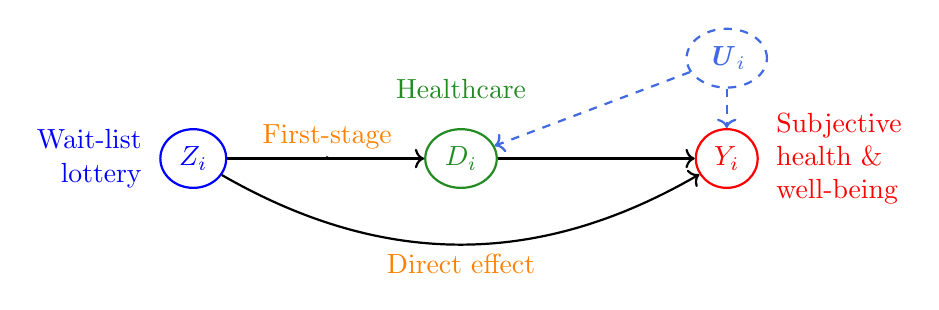
\begin{tikzpicture}
            \node[state,thick,ForestGreen] (mediator) at (0,0) {$D_i$};
            \node[state,thick,blue] (treatment) [left=2.5cm of mediator] {$Z_i$};
            \node[state,thick,red] (outcome)   [right=2.5cm of mediator] {$Y_i$};
            % Causal effects
            \path[->, thick] (treatment) edge (mediator);
            \path[->, thick] (mediator)  edge (outcome);
            \path[->, thick] (treatment) edge[bend right=30] (outcome);
            % Label Z_i, D, Y_i
            \node[color=ForestGreen] [above=0.25cm of mediator] {Healthcare};
            \node[color=blue,align=right] [left=0.1cm of treatment] {Wait-list \\ lottery};
            \node[color=red,align=left] [right=0.1cm of outcome] {Subjective \\ health \& \\ well-being};
            % Label the effect sizes.
            \node[color=black] (firststage) at ($(mediator)!0.5!(treatment)$) {.};
            \node[color=orange] [above=-0.15cm of firststage] {First-stage};
            \node[color=orange] [below=0.7cm of mediator] {Direct effect};
            \pause
            \node[state, thick,dashed,thick,RoyalBlue] (confounderU) [
                above=0.5cm of outcome] {$\vec U_i$};
            \path[->,thick,dashed,color=RoyalBlue] (confounderU) edge (mediator);
            \path[->,thick,dashed,color=RoyalBlue] (confounderU) edge (outcome);
        \end{tikzpicture}
    \end{figure}
    \vskip-0.5cm
    \par\noindent\rule{\textwidth}{0.4pt}
    \pause
    In economic settings, Conventional CM analyses have bias similar to classical selection bias \textcolor{gray}{(Heckman Ichimura Smith Todd 1998)}.
    %\hyperlink{cm-model}{\beamergotobutton{Model}}
    \begin{itemize}
        \item Direct:
        $ \;\;\ \text{\textcolor{purple}{CM Estimand}}
        = \text{\textcolor{blue}{ADE}}
            + \Big(\text{\textcolor{red}{Selection Bias}}
            + \text{\textcolor{orange}{Group difference bias}}\Big) $
        \item Indirect:
        $ \;\;\;\; \text{\textcolor{purple}{CM Estimand}}
            = \text{\textcolor{ForestGreen}{AIE}}
            + \Big(\text{\textcolor{red}{Selection Bias}}
            + \text{\textcolor{orange}{Group difference bias}}\Big). $
        \hyperlink{group-diff-ade}{\beamergotobutton{ADE biases}}
        \hfill
        \hyperlink{group-diff-aie}{\beamergotobutton{AIE biases}}
    \end{itemize}
\end{frame}
%-------------------------------------------------------------------------------
\begin{frame}
    \frametitle{Causal Mediation (CM) --- Selection Bias}
    With strategic selection, the bias terms can be large and mislead inference on how much goes through the mediating channel.
    
    \makebox[\textwidth]{\parbox{1.25\textwidth}{
        \begin{figure}
            \vskip-0.25cm
            \caption{Simulated Distribution of CM Effect Estimates from 10,000 DGPs.}
            \vskip-0.25cm
            \begin{subfigure}[c]{0.45\textwidth}
                \centering
                \caption{$\hat{\text{ADE}} - \text{ADE}$.}
                \vskip-0.25cm
                \includegraphics[width=\textwidth]{
                    ../text/sections/figures/ols-direct-dist.png}
            \end{subfigure}
            \begin{subfigure}[c]{0.45\textwidth}
                \centering
                \caption{$\hat{\text{AIE}} - \text{AIE}$.}
                \vskip-0.25cm
                \includegraphics[width=\textwidth]{
                    ../text/sections/figures/ols-indirect-dist.png}
            \end{subfigure}
        \end{figure}
    }}
\end{frame}
%-------------------------------------------------------------------------------
\section{3. CM with Selection}
\begin{frame}
    \frametitle{CM with Selection}
\end{frame}
%-------------------------------------------------------------------------------
\section{4. Return to Oregon}
\begin{frame}
    \frametitle{Oregon Health Insurance Experiment}
\end{frame}
%-------------------------------------------------------------------------------
\section{Conclusion}
\begin{frame}
    \frametitle{Conclusion}
\end{frame}
%-------------------------------------------------------------------------------
\end{document}
